Recent years have witnessed a resurgence in partisan polarization in the United States. Politically engaged citizens hold more diverging policy
views, are more ideologically extreme, and exhibit stronger negative affect towards out-partisans than in the past \citep{hetherington2001resurgent, abramowitz2008polarization, iyengar2012affect, mason2014disrespectfully, huddy2015expressive, iyengar2015fear}. A growing literature in moral psychology attributes this divide (at least partially) to fundamental differences in moral frameworks that guide liberal and conservative thinking \citep[e.g.,][]{haidt2012righteous,graham2013moral}. A recent analysis by \citet{garrett2018moral}, for example, finds that individual tendencies to moralize politics exacerbates affective polarization between Democrats and Republicans, which ultimately results in greater social distance and hostility towards out-partisans. More generally, moral conviction as an attribute of attitude strength has been shown to have wide-ranging behavioral consequences \citep{skitka2005moral,skitka2014social}, including diminishing people's willingness to compromise in the realm of politics \citep{ryan2014reconsidering,ryan2017no}.

Do these findings imply that morality in politics is always bound to foster disagreements and hostility between opposing views? Recent research building on Moral Foundations Theory pioneered by \citet{haidt2007new} and colleagues suggests otherwise. According to this view, disagreements about morality are rooted in the underlying intuitions that form people's moral frameworks \citep{haidt2012righteous}. For instance, differential emphasis on the moral foundations predicts attitudes on culturally divisive issues such as abortion, the death penalty, or same-sex marriage \citep{koleva2012tracing}. More importantly, however, ideological divides may be overcome if people speak the same ``moral language.'' Indeed, political arguments can persuade individuals holding opposing views to the extent that they are emphasizing common moral ground \citep{feinberg2015gulf}. Moral frames that rely on this logic, for example, were shown to be effective in convincing conservatives to embrace environmental protection policies and sustainable behavior \citep{kidwell2013getting,feinberg2013moral}.

However, few studies examined the persuasiveness of congruent moral appeals beyond the context of simple framing scenarios. Accordingly, the suggested potential of moral arguments to help overcoming disagreements---for example in the context of political discussions---is largely assumed as a potential implication and has not been subjected to a direct empirical test.

The present paper fills this gap by analyzing the content of more than 10,000 conversations on \texttt{/r/ChangeMyView} (CMV), an active community on the content aggregation and discussion website \textit{Reddit}.\footnote{\url{https://www.reddit.com/r/changemyview/}} Users can initiate a discussion on CMV by posting an opening statement establishing a personally held view on a particular issue (e.g., ``CMV: I believe that the gay marriage discussion isn't as important as the media portrays it to be.''), followed by a brief explanation of their underlying rationale. Other users are then invited to challenge the original poster's (OP) opinion by providing counterarguments. OPs respond to the challenges and---crucially---identify individual posts that changed their mind. The rules of the community emphasize their dedication to civil discourse and encourage OPs to be open to changing their views and identifying convincing counterarguments genuinely.\footnote{See below for more detailed information on the rules and mechanics of discussions on CMV.} This format of online discussions provides an ideal environment to explore the correlates of argument persuasiveness. In contrast to past framing studies, it allows for an examination of a wide array of issues that are viewed as important enough for people to engage in the discussion. Furthermore, the nature of the conversations on CMV as well as the anonymity of individual users turns the focus on the content and merits of arguments rather than source cues and identity-related factors. Lastly, the availability of a multitude of arguments that challenge one view allow for a unique counterfactual design of argument persuasiveness while holding many other factors constant.

The analyses in this paper rely on a dataset published by \citet{tan2016winning}. The results show that OPs who emphasize moral considerations in their opening statements are less likely to change their mind about the issue. Turning to the analysis of counterarguments, however, shows that moral appeals alone are neither beneficial nor detrimental for persuasion. Consistent with Moral Foundations Theory, persuasive arguments are characterized by a higher degree of moral congruence between the counterargument and opening statements.

% Make a convincing argument for why \texttt{/r/ChangeMyView} is a perfect case to study the effect of moral arguments in discussions and fill this gap. Describe basic idea of the subreddit. Definitely cite \citep{tan2016winning} as the data source!


\section{Theoretical Background} % NEED BETTER SECTION TITLE

Politics are about persuasion and persuasive messages. Political implications for persuasion, check one of the papers on the tablet.

\subsection{Two Routes to Persuasion}

Elaboration-Likelihood model: two different routes to persuasion \citet{petty1986elaboration}. Central route vs. peripheral route. If elaboration likelihood is low, then issue relevant thinking will be minimal. 

Moral arguments can play through both, central and peripheral routes, i.e., they can affect argument strength through central processing, but they can also have an identity-based heuristic function.

Discuss \citet{nelson2005values} and the role of values in persuasion.

The following analysis focuses more on the central route to persuasion, although emotional aspects etc. can still play a role with regard to moral appeals.


\subsection{Morality and the Potential for Compromise}

%--- Review contrasting moral foundations theory and moral conviction literature. ---

Political discussions often revolve around underlying basic principles, especially in a polarized environment. (needs citation).

Moral Psych says that people won't be persuaded if their attitudes are moralized.

% TRANSITION BETWEEN THESE TWO PARAS NEEDS WORK

Importantly, not everyone agrees with this general prediction. In fact, scholars from a different strand of literature in moral psychology have quite opposing predictions regarding the role of moral appeals in facilitating compromise. \citet{skitka2005moral} and others, for example, provide a different theoretical perspective than MFT by conceptualizing moralization as a unique feature of attitude strength. According to this view, moral convictions are perceived as ``absolutes, or universal standards of truth that others should also share'' \citep[269]{skitka2010psychology}. As such, moral convictions are viewed by individuals as applying to everyone (universality), they do not require an immediate underlying rationale but are rather seen as facts about the world (objectivity), they can be independent of authority and group norms (autonomy), they elicit strong emotional reactions, and they have an inherent motivational quality (motivation/justification) \citep{skitka2010psychology}. Building on this work, \citet{ryan2014reconsidering} argues that moral convictions are not restricted to issues that are traditionally perceived as ``moral,'' such as abortion or same-sex marriage, but can also include other issues such as economic policies. The degree of moral conviction may therefore vary between individuals as well as across issues. \citet{ryan2014reconsidering} further showed that the propensity to moralize---i.e.~the tendency to view an issue as a question of ``right and wrong''---is related to political participation, extreme political attitudes, arousal of negative emotions, and hostility. In a subsequent study, \citet{ryan2017no} suggests that moralization as a distinct characteristic of attitude intensity reorients behavior from maximizing gains to the general adherence to rules. Across multiple studies, the author shows that this tendency translates into stronger opposition to compromise about political issues and decreased support for compromising politicians. These patterns should also translate into attitudes towards---and interactions with---others who hold opposing views. Indeed, moral conviction has been shown to be related to stronger preferences for social distance from (and hostility towards) attitudinally dissimilar others and lower cooperativeness in groups holding heterogeneous views \citep{skitka2005moral}.

According to Moral Foundations Theory (MFT), liberals focus on \emph{individualizing} moral foundations, which include care/harm and fairness/cheating. Conservatives, on the other hand, also emphasize the remaining \emph{binding} foundations of loyalty/betrayal, authority/subversion, and sanctity/degradation \citep{haidt2007morality, graham2009liberals}. Differential emphasis on these moral dimensions is systematically related to attitudes towards a wide variety of divisive political issues \citep[e.g.][]{koleva2012tracing, kertzer2014moral, low2015moral}, personality traits like individual social dominance orientation (SDO) and right-wing authoritarianism (RWA) \citep{federico2013mapping}, as well as voting behavior \citep{franks2015using}. Overall, this body of research suggests that liberals and conservatives endorse different moral foundations and that these differences are closely related to political attitudes, evaluations, and behavior.

An implicit assumption in this literature is that liberals and conservatives would be more likely to come to agreements \emph{if only they focused on the same moral foundations}. For example \citet[365]{haidt2012righteous} concludes in his book \emph{The Righteous Mind: Why Good People Are Divided by Politics and Religion}: ``Once people join a political team, they get ensnared in its moral matrix. They see confirmation of their grand
narrative everywhere, and it's difficult---perhaps impossible---to convince them that they are wrong \emph{if you argue with them from outside of their matrix}'' (emphasis added). In an different article, \citet[1040]{graham2009liberals} contend that their findings ``help explain \emph{why liberals and conservatives disagree on so many moral issues} and often find it hard to understand how an ethical person could hold the beliefs of the other side: Liberals and conservatives \emph{base their moral values, judgments, and arguments on different configurations} of the five foundations.'' The underlying assumption that emphasizing the same foundations can facilitate compromise has important implications---especially in our current political environment. Somewhat surprisingly, however, this claim has never been subjected to a direct empirical test.

\subsection{Hypotheses}

Ultimately, both perspectives in moral psychology lead to diverging expectations regarding the effect of moral appeals on the potential for compromise: While the moral conviction literature suggests that \textit{any} type of moral appeal should make it harder to overcome disagreements, moral foundations theory contends that agreement can be facilitated if two discussants focus on the same underlying moral dimensions. Consider for example a discussion between person $\mathcal{A}$ who is set out to defend a specific opinion and person $\mathcal{B}$ who wants to challenge $\mathcal{A}$'s view and convince her otherwise. Suppose that $\mathcal{A}$ makes an opening statement justifying her opinion using moral arguments. Person $\mathcal{B}$ may then engage in the discussion and by trying to persuade $\mathcal{A}$ using either moralized or non-moralized counterarguments. Both theoretical perspectives described above suggest contrasting hypotheses regarding the persuasiveness of $\mathcal{B}$'s appeals:
\begin{center}\singlespacing\begin{tabularx}{\textwidth}{lX}
\textit{H1 (Moral Conviction)}: & Moralized counterarguments are going to be \textit{less} persuasive than non-moralized counterarguments.\\
\textit{H2 (Moral Foundations)}: & Moralized counterarguments that are congruent with the original argument's moral framework are going to be \textit{more} persuasive than non-moralized or morally incongruent counterarguments.
\end{tabularx}\end{center}
% HYPOTHESES NEED MORE WORK! MAKE CLEAR WITH EXAMPLE

The present paper tests both competing predictions by analyzing online discussions on the Reddit community \texttt{/r/ChangeMyView}. 

% ADD MOTIVATION WHY CHANGEMYVIEW IS THE PERFECT LABORATORY FOR DISCUSSION IN THIS CASE


\section{The Subreddit ``ChangeMyView''}
% OTHER CMV EXAMPLES:
% - Check cases 246 (discussing Haidt's theory) and 275 (on marriage equality)

Reddit is an online discussion board organized into thematic forums called \textit{subreddits}. Users can join these communities based on their interests and each subreddit has its own norms and etiquette that are enforced by voluntary moderators. \texttt{/r/ChangeMyView} (CMV) is a Reddit community where participants begin a discussion thread by stating their personal opinion on a chosen issue. Other users are invited to challenge the original posters' (OP) arguments and try to persuade them otherwise. The OPs then respond to the arguments brought forward and explicitly identify forum entries that changed their view by awarding a ``Delta'' ($\Delta$). The participation rules of the community foster civil exchange of arguments---even for divisive issues---and OPs are encouraged to award \(\Delta\)s genuinely.\footnote{The current set of rules for original posts as well as responses can be accessed at \url{https://www.reddit.com/r/changemyview/wiki/rules}. See Appendix for an overview.} To date, the subreddit has more than 500,000 subscribed users.



% ANONYMITY as an advantage? Group membership is less of an issue, the focus is on the content of the arguments themselves. -> central route rather than peripheral route

As an illustrative example, consider the following discussion on marriage equality that was posted in 2014. The thread begins with the following opening statement (the posts were slightly edited for readability):
\begin{quote}\singlespacing
\emph{CMV: I believe that the gay marriage discussion isn't as important as the media portrays it to be.}

The real problem is the concept of marriage itself. In my view, LGBT couples are already married, regardless of the legislation that is imposed on them. Marriage isn't a set of civil rights that confirms your connection to your partner, it's the choice you make to be in private, daily, lifelong commitment to another being.

Tradition dictates that in order to be `properly' married you have to exchange vows, get a ring, and have a massive celebration (the set of traditions change based upon the culture.) but marriage isn't that, it is simple commitment to another person. The main issue that gay marriage has is that not all couples are given the same civil liberties, but this does not mean that their marriages are void. Marriage isn't decided by bystanders, it's decided by the people who live inside the union. It is for this very reason that a gay couple getting married doesn't affect your own marriage.

I've held this opinion for a while but have never had the opportunity to see if it stood up to criticism. CMV.
\end{quote}
Here, the OP argues that marriage equality should be less of a controversy since the defining feature of marriage is the commitment in a relationship rather than its legal status. Several users argued against this view from various perspectives. Below is a sample response that ultimately lead the OP to award a $\Delta$ to indicate that it changed his or her view:
\begin{quote}\singlespacing
That would be true if it was just some odd tradition. But it isn't just the ceremony, but also a tax.

Right now there is a gay tax. Gay couples have to pay higher taxes than straight couples because the government gives a tax break for married couples. The reason for this is that married couples tend to be more efficient and better for the government. The government wants to encourage marriage, so as with all things they encourage they subsidize it.

Gay people provide the exact same benefits to marriage, if not more! Adoption being the largest one.

This tax comes through in multiple ways. The yearly tax and through inheritance. The government doesn't tax inheritance as much for marriage, but if they are simply partners then they get taxed when their ``partner'' dies. 

The state also doesn't allow for gay couples see their loved ones in hospitals or prison because they aren't married.

If this was just in the church I wouldn't care. But this is much more than that.
\end{quote}
However, other discussants were less successful in persuading the OP. In contrast to the previous example, the following response did not receive a $\Delta$:
\begin{quote}\singlespacing
If gay marriage is not allowed in a state
\begin{enumerate}
\item Their marriages technically \textit{are} null and void, as the state does not recognize them.
\item Marriage is not actually decided by the people in the union, since there are legal requirements as well as legal benefits. Which brings me to my next point.
\item There are several legal benefits (as well as tax benefits) to being married. States which do not allow gay marriage do not give these legal benefits to gay couples.      
\end{enumerate}
You might believe you are married to someone, but the term ``marriage'' is a political one indeed since it has legal ramifications.
\end{quote}
While both responses emphasize the importance of legal considerations in justifying the need for marriage equality, only one of the contributions persuaded the OP sufficiently such that he awarded a $\Delta$. Ultimately, these structured online discussions on CMV provide an ideal opportunity to study the persuasiveness of moral appeals. They begin with a short explanation of a person's opinion on a given topic. Multiple users attempt to counterargue the OP's point of view from various perspectives in a civil dialogue. Most importantly, OPs explicitly identify and label arguments they found to be persuasive enough to change their views.

\citet{tan2016winning} make use of this structured discussion and explore interaction dynamics on CMV by analyzing linguistic features that predict persuasiveness as well as the malleability of original posts. Their dataset includes more than 10,000 discussions that were posted on the subreddit between January 2013 and May 2015. The analyses presented below leverage the dataset compield by \citet{tan2016winning}. In this context, it is important to note that the analysis published by \citet{tan2016winning} focuses less on the content of discussions (i.e., \textit{what is being said}) but rather examined discussion dynamics and linguistic characterics (i.e., \textit{how it is expressed}) to predict persuasiveness. The following analyses explicitly turns to the effects of moral content on discussion outcomes.

% ADVANTAGES OF CMV DATA:
% - one sided argument
% - honest labeling.

Before turning to the analysis, I want to provide a brief overview of the range of topics that are discussed on CMV. Based on the set of more than 10,000 original discussion posts included in the data, I estimated a basic topic model extracting clusters of co-occurring terms via Latent Dirichlet Allocation \citet{blei2003latent}. The topic models are based on the set of original opening statements (disregarding subsequent comments), which were pre-processed by removing numbers, punctuation, symbols, hyphens, URLs, as well as stopwords. All remaining terms were stemmed and only included if they appeared in at least 10 different posts. Figure~\ref{fig:lda} displays the average topic proportions of opening statements based on the model.

\begin{figure}[ht]
\centering
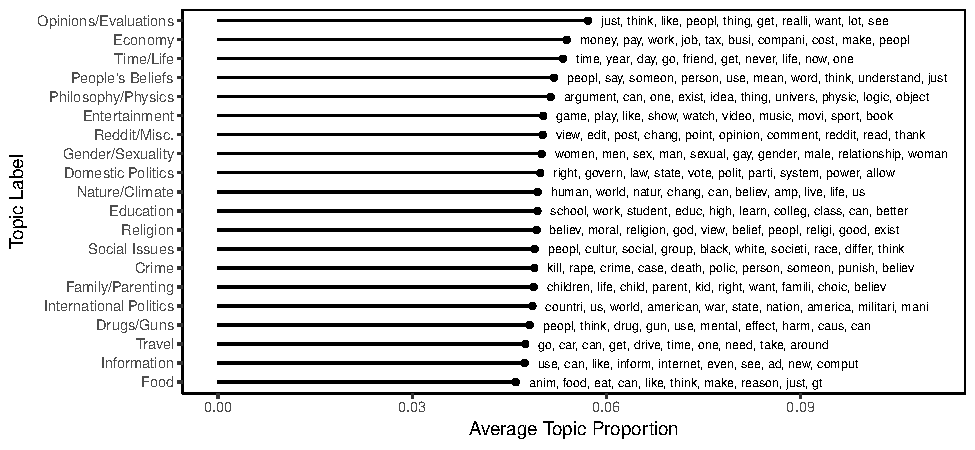
\includegraphics{/data/Dropbox/Uni/Projects/2017/cmv/calc/fig/topics.pdf}
\caption{Average topic proportions in original posts on \texttt{/r/ChangeMyView/} based on a basic LDA model with 20 topics. The plot additionally displays the ten most likely terms associated with each respective topic.}\label{fig:lda}
\end{figure}

Discussions on CMV range across a variety of topics such as economic issues, gender/sexuality, or domestic and international politics. Additional analyses included in the appendix show that there are slight differences in the extent to which topics differ in the likelihood of persuasion in discussions, although these differences are surprisingly small. The following sections turn to the role of moral appeals in facilitating or inhibiting compromise.

% ELABORATE, WHAT DOES THIS MEAN FOR RYAN'S WORK


\section{Opinion Change in Online Discussions}
%\section{Someone is Wrong on the Internet}
%\section{Do People on the Internet Change their Opinions?}
%\section{Can People on the Internet be Persuaded?}

As an initial step, I examine the extent to which OPs are willing to award $\Delta$s during a discussion in the first place. Figure~\ref{fig:delta} displays the number of discussions included in the dataset where OPs indicated that one of the responses changed their mind.

\begin{figure}[ht]
\centering
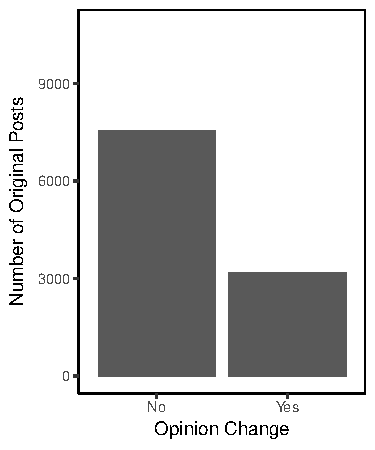
\includegraphics{/data/Dropbox/Uni/Projects/2017/cmv/calc/fig/delta.pdf}
\caption{Number of original posts on \texttt{/r/ChangeMyView/} that resulted in opinion change ($\Delta$ awarded by author) versus not.}\label{fig:delta}
\end{figure}

In about two thirds of the discussions on CMV between 2013 and 2015, OPs did not award a $\Delta$ for any of the counterarguments that were put forward, which leaves about 3,000 individual discussions where OPs indicated that at least one of the responses changed their views.

In their original study, \citet{tan2016winning} investigated linguistic and style patterns such as the use of personal pronouns as well as formatting that predicted resistance to persuasion among OPs. They conclude that ``comparative adjectives and adverbs are a sign of malleability, while superlative adjectives suggest stubbornness.'' The goal of the present analysis, however, is to go beyond pure linguistic style and explore the role of moral content in persuasion. To capture moral appeals in discussions, I rely on the the Moral Foundations Dictionary proposed by \citet{graham2009liberals}, which contains lists of word stems that signal each of the five moral foundations (care, fairness, loyalty, authority, sanctity) as well as a category of general moral terms. The full dictionary is included in Appendix A.

\begin{figure}[ht]
\centering
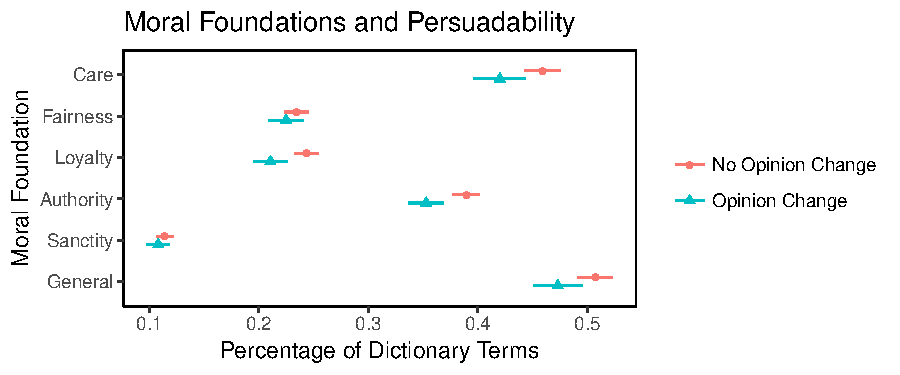
\includegraphics{/data/Dropbox/Uni/Projects/2017/cmv/calc/fig/persuadability.pdf}
\caption[Moral Foundations and Persuadability]{Moral Foundations and Persuadability: Average percentage of dictionary terms relative to the total number of words in each original post starting a discussion, comparing original posts where the author subsequently awarded a $\Delta$ (opinion change) or not (including 95\% confidence intervals).}\label{fig:persuadability}
\end{figure}

% ELABORATE ON CONSISTENCY WITH KRAFT ETC.
Figure~\ref{fig:persuadability} displays the percentage of dictionary terms belonging to each moral foundation relative to the total number of words comparing in opening statements beginning a discussion. Most importantly, the plot compares the reliance on moral terms between OPs that later reported that they changed their view versus OPs who did not. Interestingly, the distribution of dictionary terms across foundations is strikingly similar to the average proportions of moral terms in open-ended responses in the American National Election study reported in \citet{kraft2018measuring}. More importantly, the percentage of dictionary terms among opening statements that resulted in opinion change are significantly larger for two foundations, namely authority and loyalty ($p<.01$ in both cases after accounting for multiple comparisons using Bonferroni correction). OPs who did not award any $\Delta$s in the subsequent discussion put a significantly stronger emphasis on moral considerations related to loyalty and authority. We obtain a similar result after aggregating all moral dictionary terms in one category: OPs who not persuadable on CMV make stronger use of moral terms \textit{in general} than OPs who indicate that the discussion changed their view ($p<.001$). This basic result is consistent with the moral conviction literature, which posits that people who hold moralized attitudes are less willing to compromise \citep[e.g.,][]{skitka2005moral,ryan2014reconsidering,ryan2017no}.


\section{What Makes an Argument Persuasive?}
%\section{Determinants of Argument Persuasiveness}

% HOW DOES THIS RELATE TO THE SPECIFIC HYPOTHESES?

% SIGNPOST THAT I AM LOOKING FIRST AT THE OPENING STATEMENT, THEN REPLIES

However, the main interest of this paper is not the persuadability of OPs (which is certainly driven by unobserved confounding variables). Instead, we want to look at the persuasiveness of counterarguments that are made in response to the opening statements.

The previous section demonstrated that the usage of moral terms in initial statements by OPs is predictive of the malleability of their opinions. Next, I directly examine the effectiveness of specific counterarguments that were brought forward to challenge the OPs' views. \citet{tan2016winning} propose a selection of argument pairs that respond to an original post with only one being successful in changing the OPs view while being relatively similar in terms of their word choice.

{[}Elaborate on argument pair selection etc.{]}

More specifically, \citet{tan2016winning} select similar argument pairs based on their Jaccard similarity:
\begin{equation}
\text{Jaccard}(A,B)=\dfrac{|A\cap B|}{|A\cup B|},
\end{equation}
where $A$ and $B$ are the sets of words in both counterarguments. In other words, they match each successful counterargument to an unsuccessful response that shares the larges proportion of common words (disregarding stopwords).\footnote{Elaborate on additional selection criteria.} As \citet[5]{tan2016winning} describe: ``This leads to a balanced binary prediction task: which of the two lexically similar rooted path-units is the successful one?''

The analyses reported below rely on the approach implemented by \citet{tan2016winning} to select matched argument pairs. To reiterate, I therefore focus on discussions in which OPs awarded at least one $\Delta$. The response that received a $\Delta$ is then matched to another counterargument that was not successful in changing  the OPs view but is as similar as possible in terms of its vocabulary. Note that this strategy should make it difficult to find differences in the moral foundation dictionaries as argument pairs are matched based on their lexical similarity.

\begin{figure}[ht]
\centering
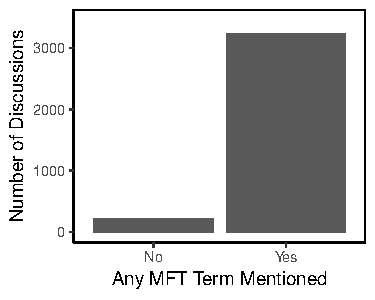
\includegraphics{/data/Dropbox/Uni/Projects/2017/cmv/calc/fig/mft_op_all.pdf}
\caption{Number of original posts in the paired argument data that included \textit{any} term mentioned in the moral foundation dictionary.}\label{fig:mft_op_all}
\end{figure}

One might worry that this selection on discussions where OPs ultimately awarded a $\Delta$ might discard all cases where the initial statement emphasized moral considerations. Luckily, that is not the case. Figure~\ref{fig:mft_op_all} shows that almost all of the opening statement in the matched pair selection mention at least one of the moral dictionary terms. Furthermore, the proportion of moral dictionary terms among this set of opening statement shows the same pattern as in Figure~\ref{fig:persuadability} (see Appendix B for details).

However, one issue that remains unresolved using this approach is that the matching procedure only focuses on the set of words that are used and does not take into account the length of each response. Figure~\ref{fig:wordcount_violin} displays the distribution of the differences in word counts between successful and unsuccessful argument pairs. Clearly, longer responses are more likely to be awarded a $\Delta$, which might be problematic when examining the effect of moral dictionary terms.

\begin{figure}[ht]
\centering
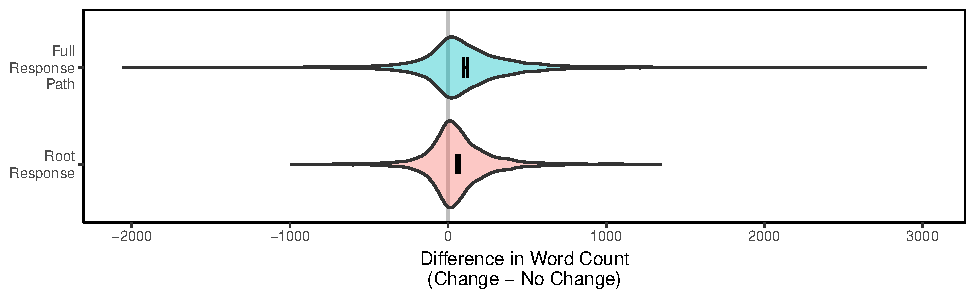
\includegraphics{/data/Dropbox/Uni/Projects/2017/cmv/calc/fig/wordcount_violin.pdf}
\caption{Difference in response lengths between successful and unsuccessful counterarguments. The narrow black bars display the 95\% confidence interval of mean differences.}\label{fig:wordcount_violin}
\end{figure}

While it could be argued that the proportion of dictionary terms should be unaffected by differences in argument length, I take additional precautions proposed by \citet{tan2016winning} to check the robustness of the results. First, I do not only examine differences when looking at the entire response path in the discussion between two users, but restrict the analysis on the initial response to the opening statement only. As can be seen in igure~\ref{fig:wordcount_violin}, the differences in word counts between argument pairs are significantly smaller. As a second step to account for the issue of response length, I additionally truncate the longer response of a given pair such that both responses contain the same number of words. Using this framework, I now turn to the analysis of the persuasiveness of moral arguments made within discussion on CMV.


\subsection{Moral Appeals are Futile...}
%\subsection{Appeals to Morality are Futile...}
%\subsection{Moral Appeals and Opinion Change}

Figure~\ref{fig:persuasiveness} displays the difference in dictionary term proportions between matched discussion contributions that were successful versus unsuccessful. Positive values indicate that arguments that received a $\Delta$ contained a larger percentage of dictionary terms, and vice versa.

\begin{figure}[ht]
\centering
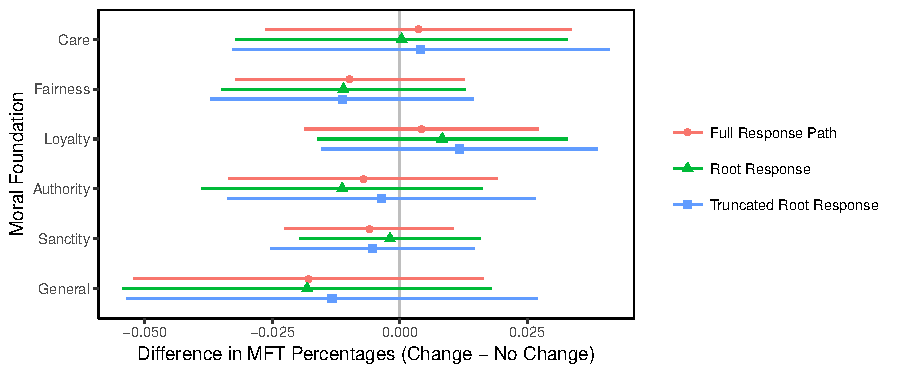
\includegraphics{/data/Dropbox/Uni/Projects/2017/cmv/calc/fig/persuasiveness.pdf}
\caption[Moral Foundations and Persuasiveness]{Moral Foundations and Persuasiveness: Average difference of dictionary term percentages relative to the total number of words in each post, comparing counterarguments where the OP subsequently awarded a $\Delta$ (opinion change) or not (including 95\% confidence intervals).}\label{fig:persuasiveness}
\end{figure}

The results show that evoking moral considerations in counterarguments does not affect the likelihood of changing the OP's view on a given issue. This result is not consistent with the moral conviction literature which would have predicted that moral appeals should in fact decrease the likelihood of compromise and opinion change.


\subsection{...Unless We're Speaking the Same Moral Language}

However, moral foundations theory argues that we cannot view moral appeals independent of the moral framework of the discussion partner. Instead, what is seen as decisive is the congruence in moral arguments between both discussants. I measure moral congruence by computing the similarity in dictionary scores between opening statements by OPs and the respective counterarguments. More formally, moral congruence is written as:
\begin{equation}
\text{moral congruence}=\dfrac{\vec{x}\cdot \vec{y}}{||\vec{x}||\hspace{.2em}||\vec{y}||},
\end{equation}
where $\vec{x}$ is the vector of dictionary counts in the OP's opening statement and $\vec{y}$ is the respective vector for a response. The measure ranges from 0 (no moral overlap) to 1 (equal emphasis on the same moral foundations).

Figure~\ref{fig:cosine} displays the difference in moral congruence between successful and unsuccessful counterarguments. Positive values indicate higher congruence in moral appeals among counterarguments that were ultimately awarded a $\Delta$ by OPs. The results clearly show that congruence in moral appeals is larger in persuasive than non-persuasive arguments.

\begin{figure}[ht]
\centering
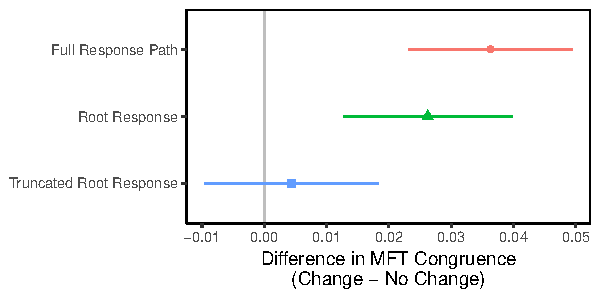
\includegraphics{/data/Dropbox/Uni/Projects/2017/cmv/calc/fig/cosine.pdf}
\caption{Moral congruence and persuasiveness: Average differences between successful and unsuccessful counterarguments in cosine similarities with the opening statements (including 95\% confidence intervals).}\label{fig:cosine}
\end{figure}

This finding is especially noteworthy since the original analysis by \citet[6]{tan2016winning} concluded that persuasive arguments used more different wording from the original post. % EXPLAIN

% ADD EXAMPLE FROM DATA IN THE END?

\section{Conclusion}\label{conclusion}

The preliminary results are consistent with moral foundations theory and contradicts the previous literature on moral convictions. While the general moralization of arguments appeared to had little effects on their persuasiveness, the results show that moral congruence with initial statements are more likely to be effective in changing a person's view. As such, moral appeals can facilitate compromise and change people's minds as long as they are consistent with their existing moral frameworks. To summarize, being able to speak the same moral language might therefore help to bridge the growing divide between liberals and conservatives.

% TALK about potential limitations: selection bias, etc.

% TO DOs, future directions, etc.:
% - examine specific topics (e.g., climate change etc.)[ ]
% - clean original posts (links etc)[x]
% - adjust confidence intervals to correct for multiple comparisons [x]
% - improve code documentation, add comments in internal functions [ ]
% - check MFT scores in argument pairs (as well as OP entry) [x]
% - take into account clustering in paired data! OPs appear multiple times [ ]


